\documentclass[10pt, compress]{beamer}

\usetheme[numbering=fraction, progressbar=none, titleformat=smallcaps, sectionpage=none]{metropolis}

\usepackage{sourcecodepro}
\usepackage{booktabs}
\usepackage{array}
\usepackage{listings}
\usepackage{graphicx}
\usepackage[brazilian]{babel}
\usepackage[scale=2]{ccicons}
\usepackage{url}
\usepackage{relsize}
\usepackage{wasysym}
\usepackage{animate}

\usepackage{pgfplots}
\usepgfplotslibrary{dateplot}

\definecolor{Base}{HTML}{191F26}
\definecolor{Accent}{HTML}{157FFF}

\setbeamercolor{alerted text}{fg=Accent}
\setbeamercolor{frametitle}{bg=Base}

\setsansfont[BoldFont={Source Sans Pro Semibold},
              Numbers={OldStyle}]{Source Sans Pro}

\lstset{ %
  backgroundcolor={},
  basicstyle=\ttfamily\footnotesize,
  breakatwhitespace=true,
  breaklines=true,
  captionpos=n,
  commentstyle=\color{orange},
  escapeinside={\%*}{*)},
  extendedchars=true,
  frame=n,
  keywordstyle=\color{Accent},
  language=C++,
  rulecolor=\color{black},
  showspaces=false,
  showstringspaces=false,
  showtabs=false,
  stepnumber=2,
  stringstyle=\color{gray},
  tabsize=2,
  keywords={thrust,plus,device_vector, copy,transform,begin,end, copyin,
  copyout, acc, \_\_global\_\_, void, int, float, main, threadIdx, blockIdx,
  blockDim, if, else, malloc, NULL, cudaMalloc, cudaMemcpy, cudaSuccess,
  cudaGetLastError, cudaDeviceSynchronize, cudaFree, cudaMemcpyDeviceToHost,
  cudaMemcpyHostToDevice, const, data, independent, kernels, loop,
  fprintf, stderr, cudaGetErrorString, EXIT_FAILURE, for, dim3, pthread_t,
  pthread_create, exit, pthread_exit, long, printf, omp, parallel, private,
  default, shared, task, taskgroup, taskloop, num_tasks,
  omp_get_thread_num, omp_get_num_threads},
  otherkeywords={::, \#pragma, \#include, \#define, <<<,>>>, \&, \*, +, -, /, [, ], >, <}
}

\renewcommand*{\UrlFont}{\ttfamily\smaller\relax}

\graphicspath{{../img/}}

\title{Introdução a Pthreads \& OpenMP}
\author{\footnotesize Pedro Bruel \\ {\scriptsize \emph{phrb@ime.usp.br}}}
\institute{
\includegraphics[height=2cm]{imelogo}\\[0.2cm] Instituto de Matemática e Estatística \\ Universidade de São Paulo}
\date{\scriptsize \today}

\begin{document}

\maketitle

\section*{Introdução}

\subsection*{Sobre o EP1}

\begin{frame}
    \frametitle{Sobre o EP1}
    Na aula passada faltou:

    \begin{itemize}
        \item Data de Entrega do EP1: \alert{25/04}
        \item Demonstrar GNU \texttt{screen}
    \end{itemize}
\end{frame}

\subsection*{Roteiro}

\begin{frame}
    \frametitle{Roteiro}
    \setbeamertemplate{section in toc}[sections numbered]
    \tableofcontents[hideallsubsections]
\end{frame}

\begin{frame}
    \frametitle{Slides}
    \begin{center}
        
\includegraphics[width=.18\textwidth]{github}
    \end{center}
    Os slides e todo o código fonte estão no \alert{GitHub}:

    \begin{itemize}
        \item \url{github.com/phrb/aula-pthreads-openmp}
    \end{itemize}
\end{frame}

\section{Motivação}

\begin{frame}
    \frametitle{Programação Concorrente: Motivação}
    Por que usar programação concorrente?

    \alert{Desempenho}:
    \begin{itemize}
        \item Arquiteturas paralelas
        \item Memória Compartilhada
        \item SMP, hyperthreaded, multi-core, NUMA, $\dots$
    \end{itemize}

    \alert{Modelagem}:
    \begin{itemize}
        \item Descrever paralelismo natural
        \item Tarefas independentes
    \end{itemize}
\end{frame}

\begin{frame}
    \frametitle{Programação Concorrente: Motivação}
    \begin{center}
        
\includegraphics[width=.55\textwidth]{shared_work}
    \end{center}
\end{frame}

\begin{frame}
    \frametitle{Programação Concorrente: Motivação}
    \begin{center}
        \animategraphics[loop,autoplay,width=\linewidth]{12}{puppies/puppies-}{0}{68}
    \end{center}
\end{frame}

\section{IEEE POSIX Threads}

\subsection{Processos \& Threads}

\begin{frame}
    \frametitle{IEEE POSIX Threads}

    \alert{IEEE} \& \alert{POSIX}:
    \begin{itemize}
        \item Institute of Electrical and Electronics Engineers (\alert{IEEE})
        \item Portable Operating System Interface (\alert{POSIX})
    \end{itemize}

    \pause

    \alert{IEEE POSIX Threads}:
    \begin{itemize}
        \item Define um \alert{modelo de execução}
        \item \alert{Independente} de linguagens
        \item Execução paralela de ``\alert{fluxos de trabalho}'' (\alert{threads})
        \item Define uma API para \alert{criação e controle} de threads
        \item \alert{Não define} detalhes de implementação
    \end{itemize}
\end{frame}

\begin{frame}
    \frametitle{Processos \& Threads}
    \begin{center}
        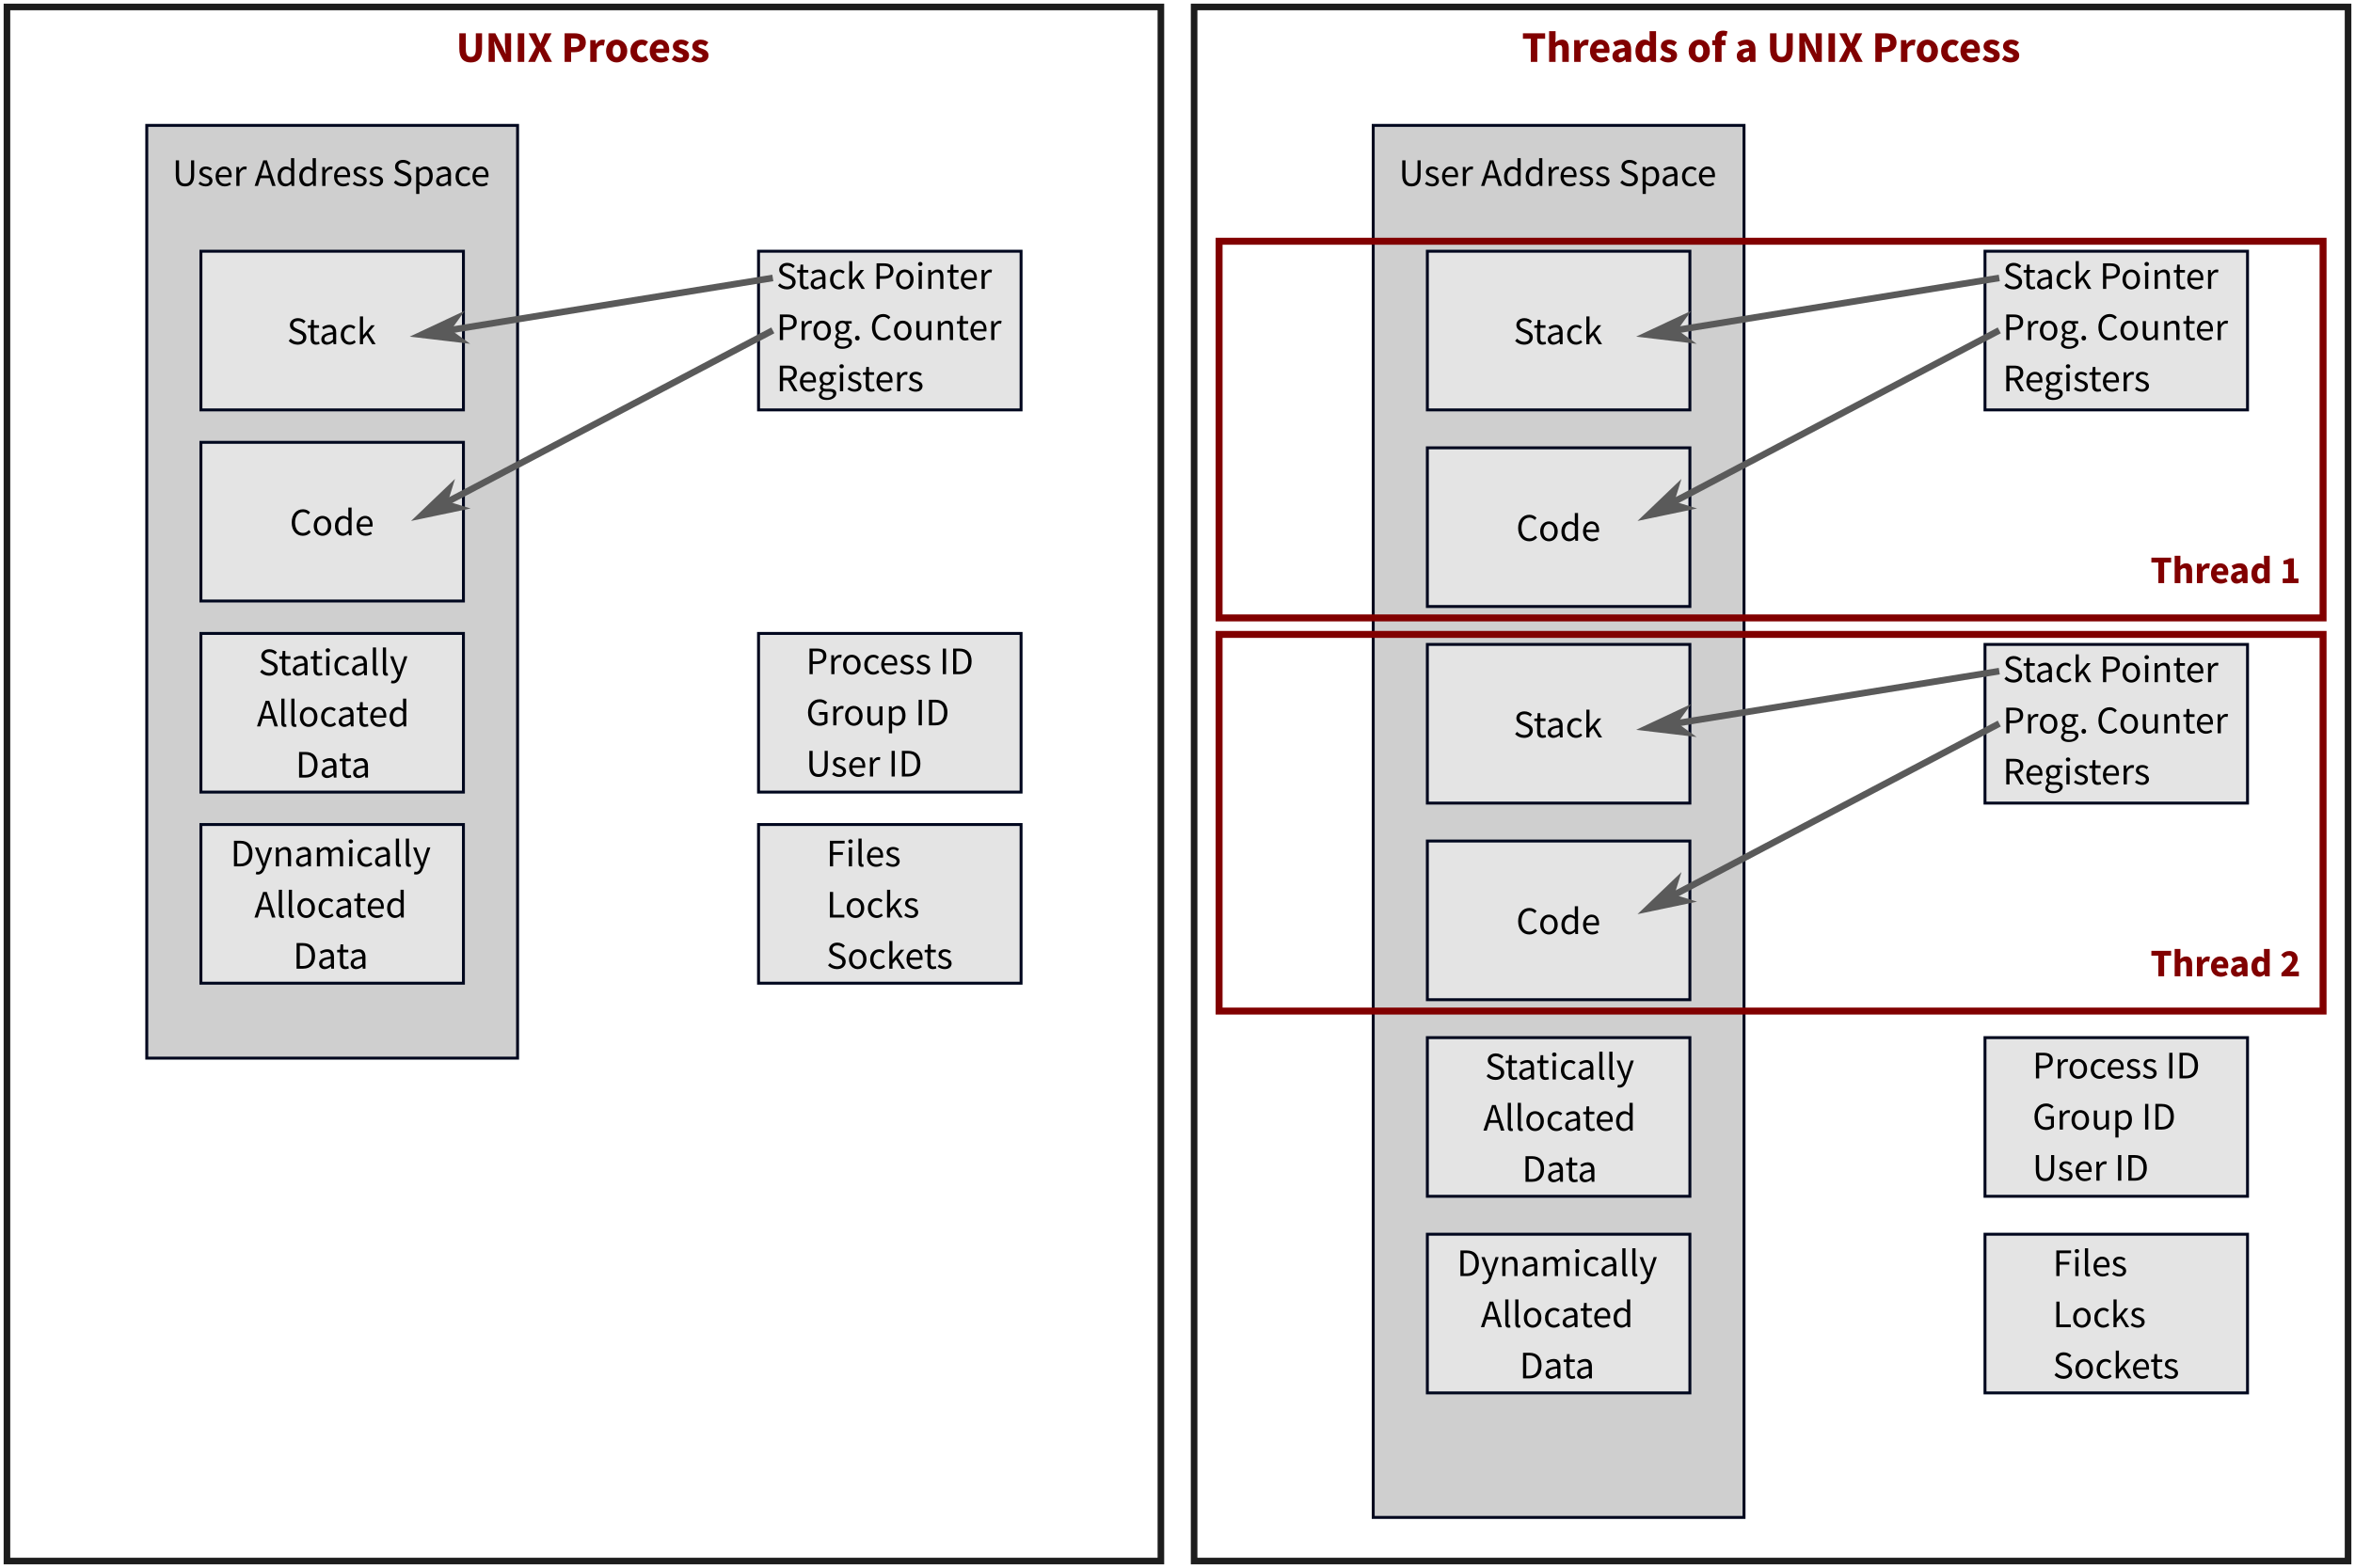
\includegraphics[width=\textwidth]{process-and-thread}
    \end{center}
\end{frame}

\begin{frame}
    \frametitle{Pthreads API}
    \alert{\textasciitilde{}100 funções} prefixadas por \texttt{pthread\_}:
    \begin{itemize}
        \item Gerenciamento
        \item Mutexes
        \item Variáveis condicionais
        \item Sincronização
    \end{itemize}
\end{frame}

\begin{frame}
    \frametitle{Pthreads API}
    \begin{table}[]
        \centering
        \begin{tabular}{@{}ll@{}}
            \toprule
            \textbf{Prefixo} & \textbf{Funcionalidade} \\ \midrule
            \texttt{pthread\_} &  Gerenciamento \\
            \texttt{pthread\_attr\_} & Atributos \\
            \texttt{pthread\_mutex\_} &  Mutexes \\
            \texttt{pthread\_mutexattr\_} & Atributos de Mutexes \\
            \texttt{pthread\_cond\_} & Variáveis condicionais \\
            \texttt{pthread\_condattr\_} & Atributos de condicionais \\
            \texttt{pthread\_key\_} & Dados específicos de threads \\
            \texttt{pthread\_rwlock\_} & \textit{Locks} de leitura e escrita \\
            \texttt{pthread\_barrier\_} &  Barreiras e sincronização \\ \bottomrule
        \end{tabular}
        \label{my-label}
        \caption{Algumas funções da API Pthreads}
    \end{table}
\end{frame}

\subsection{Exemplos}

\begin{frame}
    \frametitle{Pthreads: Tutorial}
    \alert{POSIX Threads Programming}:
    \begin{itemize}
        \item Blaise Barney, Lawrence Livermore National Laboratory
        \item \url{https://computing.llnl.gov/tutorials/pthreads}
    \end{itemize}
\end{frame}

\begin{frame}[fragile]
    \frametitle{POSIX Threads: Hello, World!}
    \begin{lstlisting}[basicstyle=\ttfamily\scriptsize]
    #include <pthread.h>
    #include <stdio.h>
    #include <stdlib.h>
    #define NUM_THREADS 5
    void *print_hello(void *threadid){
        long tid;
        tid = (long) threadid;
        printf("Hello World! It's me, thread #%ld!\n", tid);
        pthread_exit(NULL);
    };
    int main(int argc, char *argv[]){
        pthread_t threads[NUM_THREADS];
        int error_code;
        long t;
        for(t = 0; t < NUM_THREADS; t++){
            printf("In main: creating thread %ld\n", t);
            error_code = pthread_create(&threads[t], NULL,
                                        print_hello, (void *) t);
            if (error_code){
                printf("ERROR pthread_create(): %d\n", error_code);
                exit(-1);
            };
        };
        pthread_exit(NULL);
    };
    \end{lstlisting}
\end{frame}

\begin{frame}
    \frametitle{POSIX Threads: Mais Exemplos}
    Exemplos em \url{https://github.com/phrb/aula-pthreads-openmp}:
    \begin{itemize}
        \item Hello, World!
        \item Argumentos
        \item \textit{Join}
        \item Servidor IRC: \url{https://github.com/phrb/simple-irc-server}
    \end{itemize}
\end{frame}

\section{OpenMP}

\maketitle

\begin{frame}
    \frametitle{Roteiro}
    \setbeamertemplate{section in toc}[sections numbered]
    \tableofcontents[hideallsubsections]
\end{frame}

\begin{frame}
    \frametitle{Slides}
    \begin{center}
        
\includegraphics[width=.18\textwidth]{github}
    \end{center}
    Os slides e todo o código fonte estão no \alert{GitHub}:

    \begin{itemize}
        \item \url{github.com/phrb/aula-pthreads-openmp}
    \end{itemize}
\end{frame}

\begin{frame}
    \frametitle{OpenMP}
    \alert{Open Multi-Processing} (OpenMP):
    \begin{itemize}
        \item API para paralelismo \alert{multithreaded} e de \alert{memória
            compartilhada}
        \item \alert{Diretivas de compilador}
        \item Biblioteca de \alert{Tempo de Execução} (\alert{Runtime})
        \item Variáveis de ambiente
    \end{itemize}

    \pause

    Objetivos:
    \begin{itemize}
        \item \alert{Padronizar}
        \item \alert{Simplificar}
        \item \alert{Facilitar o uso}
        \item \alert{Permitir portabilidade}
    \end{itemize}
\end{frame}

\subsection{Modelo de Programação}

\begin{frame}
    \frametitle{OpenMP: Modelo de Programação}
    \begin{itemize}
        \item Threads \alert{dinâmicas}
        \item Paralelismo \alert{explícito e aninhável}
        \item \alert{Diretivas} de compilador
        \item Modelo \alert{Fork-Join}
        \item I/O e memória?
    \end{itemize}
\end{frame}

\begin{frame}
    \frametitle{OpenMP: Fork-Join}
    \begin{center}
        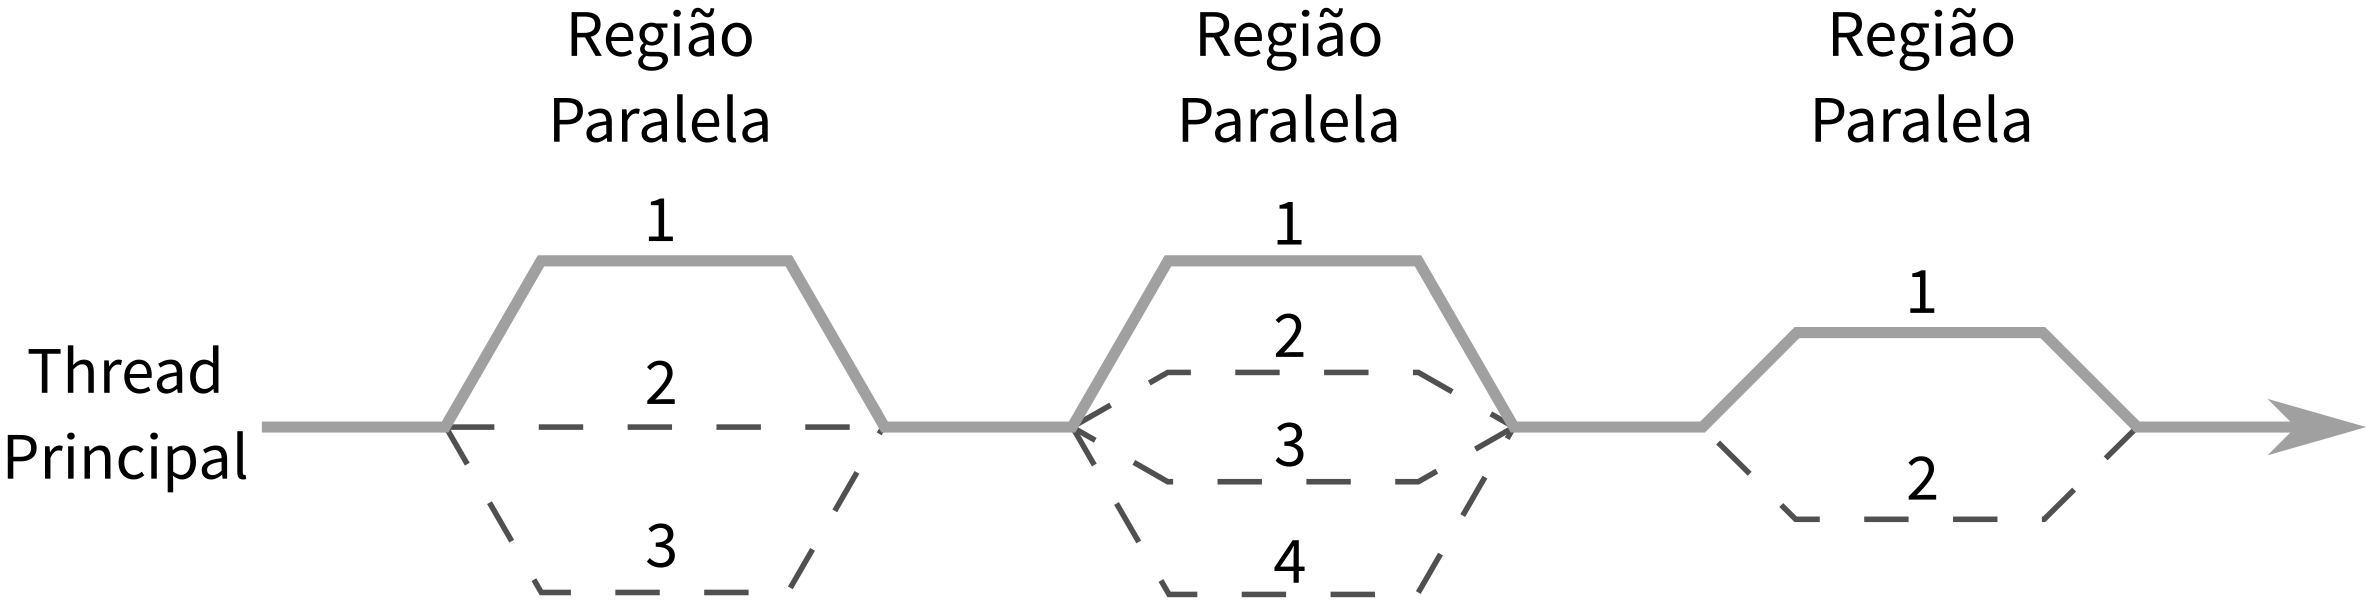
\includegraphics[width=\textwidth]{omp-fork-join}
    \end{center}
\end{frame}

\begin{frame}[fragile]
    \frametitle{OpenMP: Diretivas}
    Usadas para:
    \begin{itemize}
        \item Criar \alert{regiões paralelas}
        \item Distribuir \alert{blocos de código}
        \item Distribuir \alert{iterações de laços}
        \item \alert{Sincronizar threads}
        \item $\dots$
    \end{itemize}

    Modelo:
    \begin{lstlisting}[basicstyle=\ttfamily\scriptsize]
        #pragma omp directive [clause, ...]
    \end{lstlisting}

    Exemplo:
    \begin{lstlisting}[basicstyle=\ttfamily\scriptsize]
        #pragma omp parallel default(shared) private(beta,pi)
    \end{lstlisting}
\end{frame}

\begin{frame}[fragile]
    \frametitle{OpenMP: Biblioteca Runtime}
    Usadas para:
    \begin{itemize}
        \item Obter e definir \alert{número de threads}
        \item Obter \alert{IDs de threads}
        \item Obter \alert{região paralela e nível de aninhamento}
        \item Obter, criar e destruir \alert{locks}
        \item $\dots$
    \end{itemize}

    Exemplo:
    \begin{lstlisting}[basicstyle=\ttfamily\scriptsize]
        #include <omp.h>
        int omp_get_num_threads(void)
    \end{lstlisting}
\end{frame}

\begin{frame}[fragile]
    \frametitle{OpenMP: Variáveis de Ambiente}
    Usadas para:
    \begin{itemize}
        \item Definir \alert{número de threads}
        \item Distribuir \alert{iterações de laços}
        \item Associar \alert{threads a processadores}
        \item Configurar \alert{paralelismo aninhado}
        \item Configurar \alert{threads dinâmicas}
        \item $\dots$
    \end{itemize}

    Exemplo:
    \begin{lstlisting}[basicstyle=\ttfamily\scriptsize]
        export OMP_NUM_THREADS=8
    \end{lstlisting}
\end{frame}

\subsection{Exemplos}

\begin{frame}
    \frametitle{OpenMP: Tutorial}
    \alert{OpenMP Programming}:
    \begin{itemize}
        \item Blaise Barney, Lawrence Livermore National Laboratory
        \item \url{https://computing.llnl.gov/tutorials/openMP}
    \end{itemize}
\end{frame}

\begin{frame}[fragile]
    \frametitle{OMP: Hello, World!}
    \begin{lstlisting}[basicstyle=\ttfamily\scriptsize]
    #include <stdio.h>
    #include <omp.h>

    int main(int argc, char *argv[]){
        int nthreads, tid;

        #pragma omp parallel private(tid)
        {
            tid = omp_get_thread_num();
            printf("Hello World from thread = %d\n", tid);

            if(tid == 0){
                nthreads = omp_get_num_threads();
                printf("Number of threads = %d\n", nthreads);
            };
        };
        return 0;
    };
    \end{lstlisting}
\end{frame}

\begin{frame}
    \frametitle{OpenMP: Mais Exemplos}
    Exemplos em \url{https://github.com/phrb/aula-pthreads-openmp}:
    \begin{itemize}
        \item Hello, World!
        \item Parallel \texttt{for}
        \item Reduction
        \item Critical section
    \end{itemize}
\end{frame}

\begin{frame}
    \frametitle{OpenMP 4.5}
    Versão \alert{4.5} da \alert{API OpenMP}:
    \begin{itemize}
        \item Lançada em \alert{Novembro de 2015}
        \item OpenMP \alert{Architecture Review Board} (ARB)
        \item Requer \alert{GCC 6}:
            \begin{itemize}
                \item Xeon Phi
                \item Algumas GPGPUs AMD
                \item GPGPUs Nvidia no futuro
            \end{itemize}
        \item \alert{Especificação completa} da API no repositório
    \end{itemize}
\end{frame}

\begin{frame}[fragile]
    \frametitle{OpenMP 4.5: Exemplo com \texttt{taskloop}}
    \alert{Dividir e sincronizar} $1024$ iterações de um laço entre $32$
    \textit{threads}, usando \alert{OpenMP $<$ 4.5}:

    \begin{lstlisting}[basicstyle=\ttfamily\scriptsize]
    #pragma omp taskgroup
    {
        for(int tmp = 0; tmp < 32; tmp++){
            #pragma omp task
            for(long l = tmp * 32; l < tmp * 32 + 32; l++){
                do_something (l);
            };
        };
    };
    \end{lstlisting}
\end{frame}

\begin{frame}[fragile]
    \frametitle{OpenMP 4.5: Exemplo com \texttt{taskloop}}
    \alert{Dividir e sincronizar} $1024$ iterações de um laço entre $32$
    \textit{threads}, usando \alert{OpenMP $\geq$ 4.5}:

    \begin{lstlisting}[basicstyle=\ttfamily\scriptsize]
    #pragma omp taskloop num_tasks(32)
    for (long l = 0; l < 1024; l++){
        do_something(l);
    };
    \end{lstlisting}

    \pause

    Para saber mais, no \alert{blog da RedHat}:
    \begin{center}
        \scriptsize{\url{https://developers.redhat.com/blog/2016/03/22/what-is-new-in-openmp-4-5-3/}}
    \end{center}
\end{frame}

\maketitle

\end{document}
